% -*- mode: latex; mode: auto-fill; coding: utf-8; -*-

In this chapter we will introduce the helper tools implemented. The
different kind of modifiers will be introduced followed by the tensor
visualization tool.

\section{Modifiers}
\label{sec:modifiers}
The initial state of the physics system is equilibrium. In order to
simulate a reaction something has to act on the system forcing
it out of equilibrium. All interaction with the system is done
through modifiers of different types.
%
Each modifier consists of a nodal
selection tool and an action that will be applied to the selected
nodes.     
%
Any volumetric shape can be used as a selection tool. By default box
selection is used. Nodes inside the volumetric shape are in the set of 
selected nodes. During simulation a specified action is applied to the
set of selected nodes.
%
The modifiers vary in the way they interact with the physics
system. The following modifiers types will be introduced:

\begin{itemize}
\item Fixed Displacement Modifier
\item Force Modifier
\item Displacement Modifier
\item Restrictive Displacement Modifier
\item Projective Displacement Modifier
\end{itemize}

\subsection{Fixed Displacement Modifier}
The \defit{fixed displacement modifier} restrains the
displacement of all selected nodes by fixing their position in
space. The positional restriction is applied to all selected
nodes. Usually it is
necessary to restrict part of the object when external forces are
applied. Otherwise the object would just move instead of causing
deformation, but of course this depends on the scenario. 
The fixed displacement modifier is like a clamp holding
the object in place while working on it. \\

Figure \vref{fig:modifiers_fixed} illustrates a beam fixed in one
end. The fixed displacement modifier is always visualized with a green
color to indicate that the selected nodes are neutral to any stress
and strain. The restriction
is applied simply by overwriting the new displacement by the current
hereby resetting any nodal movement.

\begin{figure}
  \centering
  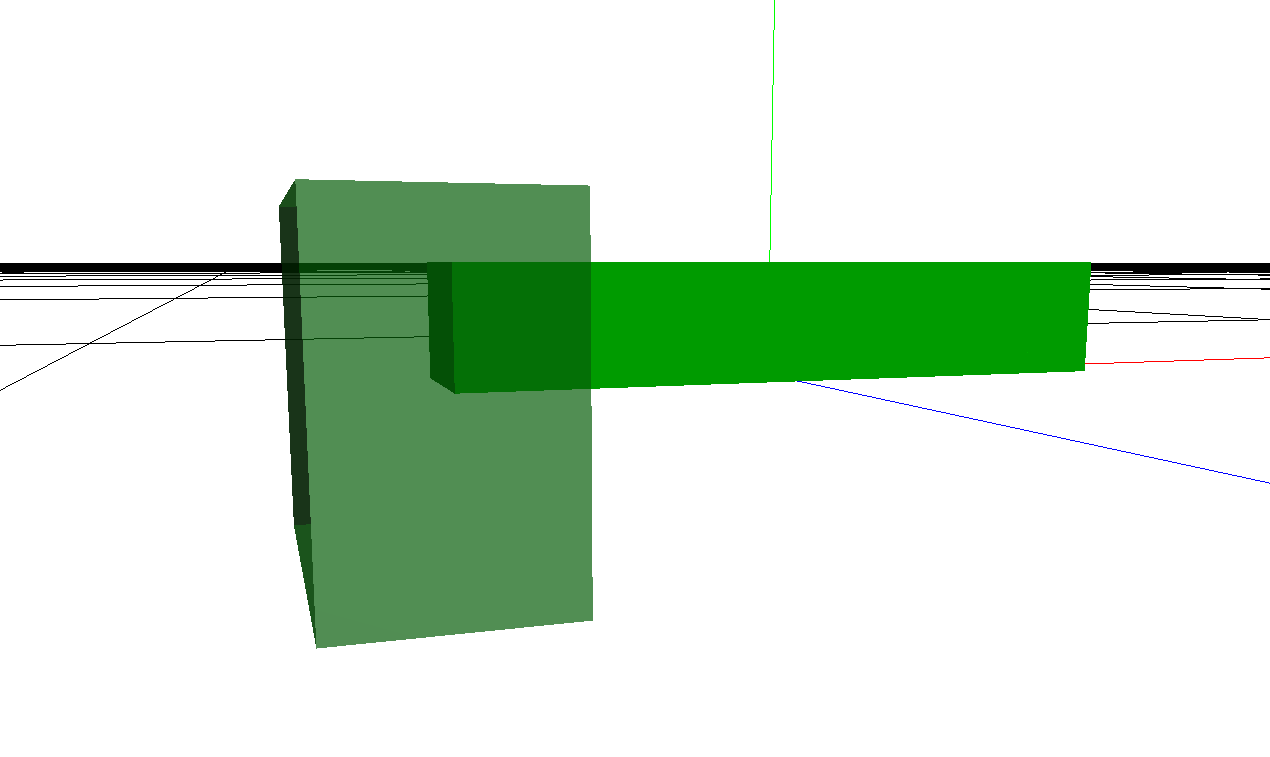
\includegraphics[width=12cm]{./images/helper_tools_modifiers_fixed.png}
\caption{Beam fixed at one end.}
\label{fig:modifiers_fixed}
\end{figure}


\subsection{Force Modifier}
The \defit{force modifier} applies a force with any specified direction and magnitude to
all selected nodes. This is very useful for applying loads to
selected parts of the object being simulated. During simulation new nodal
selection can be made hereby gradually increasing or decreasing the load.

\begin{figure}
  \centering
  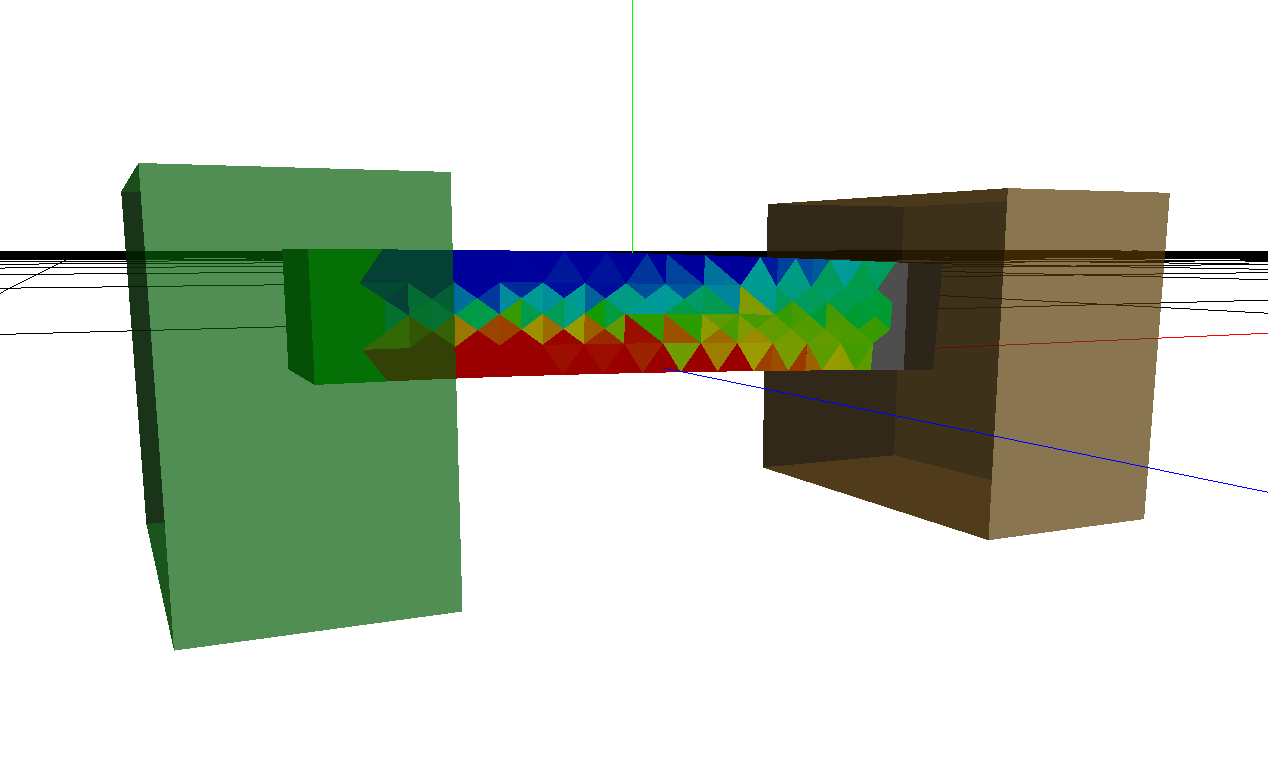
\includegraphics[width=12cm]{./images/helper_tools_modifiers_force.png}
\caption{Supported beam with load applied to its end point.}
\label{fig:modifiers_force}
\end{figure}

Figure \vref{fig:modifiers_force} illustrates a beam supported at the
left end and applied with external forces at its right end. The selection tool for the
force modifier is always visualized by a brown color with the
selected nodes grayed out. As illustrated in figure
\vref{fig:modifiers_force} only the end of the beam is selected and the
force modifier applies a force acting downwards which causes tension
on top of the beam and compression at the bottom. 


\subsection{Displacement Modifier}
The \defit{displacement modifier} adds a specified displacement vector
to all nodes selected. Furthermore it restricts the selected part of the object
from any deformation hereby preventing it from absorbing any stress or
strain. 

\begin{figure}
\label{fig:modifier_displacement}
  \centering
  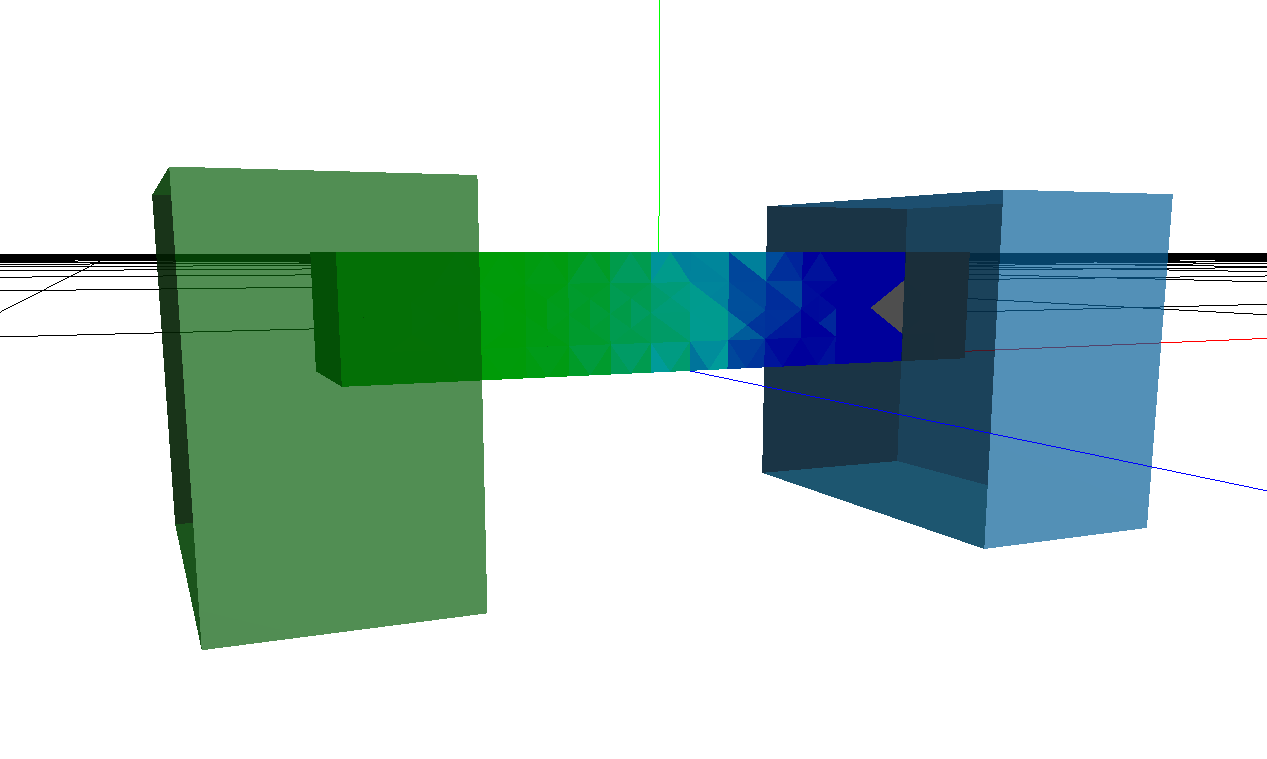
\includegraphics[width=12cm]{./images/helper_tools_modifiers_displacement.png}
\caption{The beam is fixed at the left end while stretched by the
  modifier at the other end.}
\end{figure}

Figure \vref{fig:modifier_displacement} illustrates a beam with its left
end fixed while a displacement modifier is applied at the right
end. The displacement modifier stretches the beam horizontally causing
tension in the beam. The
stresses and strains occurring as a result to this, can only occur in
the mid subsection of the beam where none of the two modifiers are
applied. The selection tool for the displacement modifier is always
visualized by a blue color with the selected nodes grayed out.


\subsection{Restrictive Displacement Modifier}
The \defit{restrictive displacement} modifier simply restricts any nodes from
entering the space occupied by the selection tool. This modifier can be
use for simple collision detection between an object and the
modifier. The restrictive displacement modifier can be used as a
ground restriction in the scene or simply as a colliding object as
illustrated in figure \vref{fig:modifier_restrictive}. If a node is
about to enter the space 
occupied by the selection tool it will be moved back to its previous
location. The drawback of this very
simple restriction is that the method only applies under the
assumption that a previous nodal position exist. If an object does not
move, all nodal positions in the current configuration at time $t$
equals the nodal positions in the previous configuration at time
$t - \Delta t$. 
%
In other words the object has to intersect with the modifier and not
the other way around. Due to the simplicity this type of modifier is
computationally fast in contrast to the projection displacement modifier
as explained next.

\begin{figure}
  \centering
  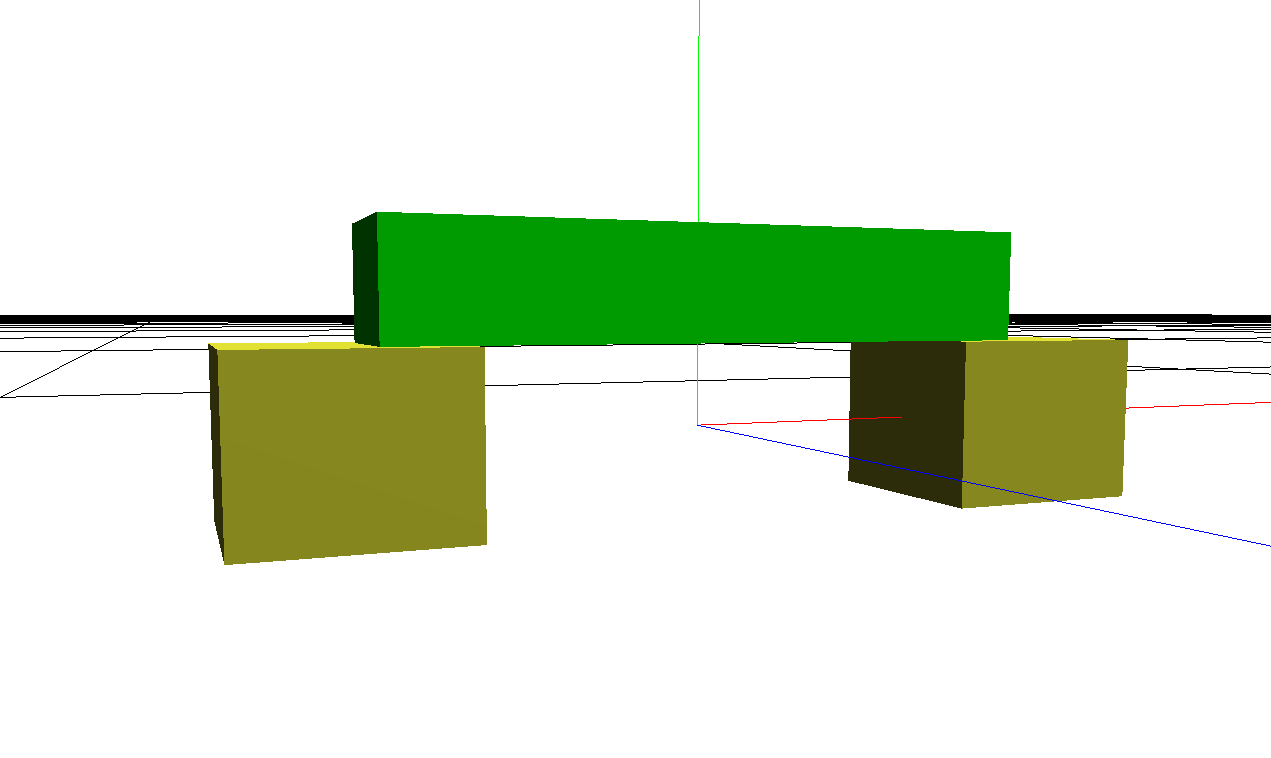
\includegraphics[width=12cm]{./images/helper_tools_modifiers_restrictive.png}
\caption{Gravitational force acts on the beam supported in both ends.}
\label{fig:modifier_restrictive}
\end{figure}

Figure \vref{fig:modifier_restrictive} illustrates the gravitational
force acting on the beam supported by two restrictive displacement
modifiers. The selection tool occupying the restrictive space is
always visualized by a yellow color.  

\subsection{Projection Displacement Modifier}
The \defit{projection displacement modifier} is an extension to the
restrictive displacement modifier, the only difference being 
the algorithm used when correcting the nodal displacements. 

\begin{figure}
  \centering
  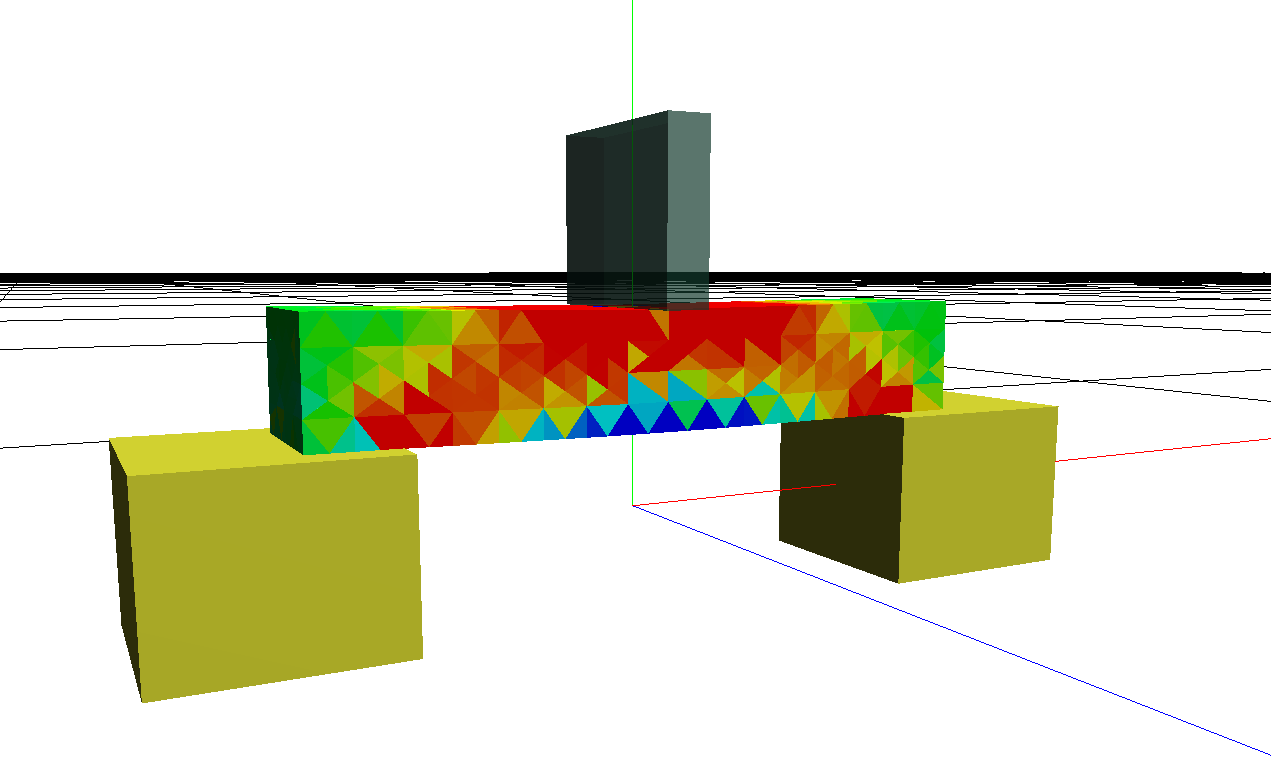
\includegraphics[width=12cm]{./images/helper_tools_modifiers_projection.png}
\caption{Center nodes at the top of the beam are forced down
  causing the beam to bend.}
\label{fig:modifier_projection}
\end{figure}

As already mentioned the
restrictive displacement modifier only works when 
the object intersects with the modifier. 
We need the ability to
interact with the object in the way a craftsman uses his tools on
a material. When the modifier intersects with an object we need to 
calculate a new displacement for the intersecting nodes.
The default strategy implemented relies on vector projection. Any node
intersecting the space occupied by the selection tool is projected
onto the closest plane from the geometry defining the selection tool.
By default a box is implemented as the selection tool. If a node
is located inside the box, the distance to each of the six planes
defining the box is calculated. The node is then projected onto the
plane closest to the node. \\

Figure \vref{fig:modifier_projection} illustrates a supported beam
being subjected to a projection displacement modifier forcing the
midpoint nodes down causing the beam to bend. The selection tool for
the restrictive displacement modifier is visualized by a dark
blue-gray color.

\section{Tensor Field Visualization}
Visualizing the stresses and strains would reveal very interesting
information e.g. how stress and strain propagates through the
simulated object and where potential strengths and weaknesses would be
located within the material. 
%
Stress and strain tensors are defined for each element. The number of
elements depends on the size 
of the problem domain but it is not unusual to have hundreds or
thousands of elements. The data set, containing a tensor for each
element forming a tensor field, can easily become relatively
large. The challenge of tensor 
field visualization is to transform this large data set into a single
image, easy to interpreted. A method for this has been presented by
\citeabook{article:tensor_visualization}. The method presented is based 
upon \defit{data transformation} and \defit{data reduction}. \\

% data transformation
Data transformation is necessary since the data set consists of tensors on
matrix form which cannot be visualized directly. We are interested in
retrieving the relevant information from the data set and represent it
differently. As already explained in section
\vref{sec:principal_values_and_directions} the eigenproblem of a
second order symmetric tensor defines the principal eigenvalues and
corresponding eigenvectors. Retrieving the principal values and
directions from a second order tensor is an example of data
transformation. \\ 

% data reduction
Data reduction is necessary since the data set can become relatively
large dependent on the size of the problem domain.  
A way of reducing the data set
could be to only extract the largest eigenvalue and the corresponding
eigenvector since these define the maximum principal value and
direction, respectively. 
%
Experiments with stress visualization indicate that when external
forces are applied to an object the amount of stress heading in the
maximum principal stress direction is by far the most dominant in comparison
to the other two stress directions. Recall that the tensor quantity (here
being stress or strain) can be resolved into three mutually perpendicular
vectors known as the maximum, medium and minimum principal
directions. \\ 

The following tensor field visualization is based upon solving the
eigenproblem for each stress tensor and reduce this by only
considering the largest eigenvalue (maximum principal stress) and the direction of the
corresponding eigenvector (maximum principal stress direction). 
The eigenvalue is visualized by
mapping it to a color scheme and the eigenvector is visualized by a
small visual entity pointing in the same direction as the eigenvector.


\subsection{Vizualizing the Eigenvalues}
%what are we trying to visualize
To visualize the maximum principal stress, we use a
color scheme. Since the eigenvalue is mapped to a color scheme which
has three components the conversion is not straightforward.
We need to use a color ramp to do the mapping.
%
%what is a color ramp
A \defit{color ramp} %\footnote{\url{http://local.wasp.uwa.edu.au/~pbourke/texture_colour/colourramp/}}
is a function which maps a range of scalar values
to colors. We use a linear scaled color ramp known as the
\defit{hot-to-cold color ramp}, ranging from blue over green to
red as illustrated in figure \vref{fig:cr-scala}. This color ramp is
ideal when visualising values above and below zero.
%\{oleby}{det er vel egentlig cold-to-hot}

\begin{figure}
  \centering
  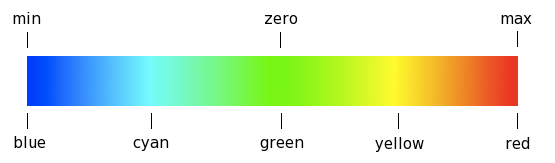
\includegraphics[width=10cm]{./images/helper_tools_color_ramp_scala.png}
\caption{The hot-to-cold color ramp.}
\label{fig:cr-scala}
\end{figure}

%how do the color values rgb work
To define such a function we first have to specify how to represent
colors in the simulation. We used the three component color scheme,
with red, green, and blue (RGB) represented as floating point values
ranging from $0$ to $1$. Any color representable is a mixture of these three
components. 
%
The three components are bundled in a $3 \times 1$ vector. So red for
example is represented as (1,0,0), green (0,1,0), and blue (0,0,1).
%
A color ramp can be illustrated as in
figure \vref{fig:cr-box}. The edge length of the box is one hereby
limiting each RGB component range to be between $0$ and $1$.
The black emphasized line in the figure illustrates the hot-to-cold
color ramp. All values are mapped to this line hereby being mapped
a scalar value to three vector components. 

\begin{figure}
  \centering
  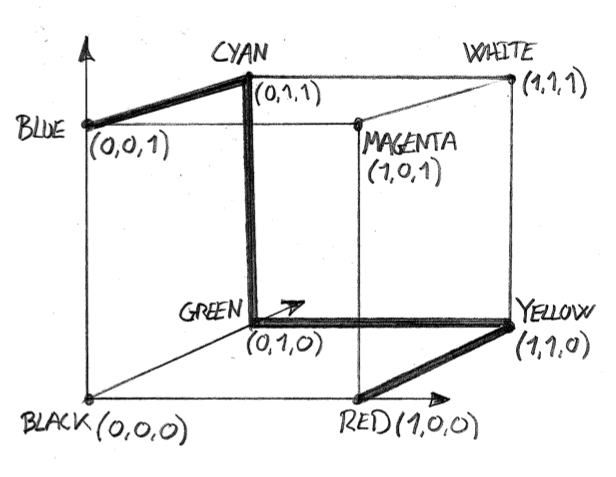
\includegraphics[width=10cm]{./images/helper_tools_color_ramp_box.png}
\caption{Illustration of how to interpolate color values for the hot-to-cold color ramp.}
\label{fig:cr-box}
\end{figure}

The principal stress is mapped to at color within the range of the
material dependent tensile strength ($\sigma^+_F$) and compressive
strength ($\sigma^-_F$). Zero stress is green, stress above
$\sigma^+_F$ is clamped to blue and stress below $\sigma^-_F$ to red.
Two linear interpolation functions are used in between, one for stretch and
one for compression. Each interpolation function is determined by the
material properties entered. 

% \{When we calculate the color of a principle stress magnitude, the
% limits for the color ramp is set the breaking point of the material
% (fracture point), as this is different for the stretch and compression
% we have two values that goes into the color ramp equation. a max and
% min value. This effectively produces two linear interpolations at each
% side of zero, with different ranges. If the maximum principle stress
% magnitude exceeds the min and max level, the color values are clamped
% to either red or blue depending on which end of the ramp we are
% talking about.}

%\subsection{Data Transformation and Reduction in Parallel}
\subsection{Visualizing the Eigenvectors}
The shape of the visual entity is important, it has to clearly illustrate the
direction and location of the stresses without requiring too many
resources. A relatively simple visual entity must be used since the size of
the tensor field grows linearly with the number of visual
elements. Figure \vref{fig:tensor_visual_flight} illustrates the shape
of the visual entity we constructed.
%
It is suitable
for visualizing the directions of the stress tensors due to its simple
representation and the obvious orientation. 

\begin{figure}
  \centering
  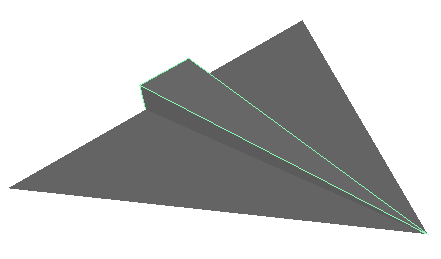
\includegraphics[width=6cm]{./images/helper_tools_tensor_flight.png}
\caption{A visual entity shaped like an airplane.}
\label{fig:tensor_visual_flight}
\end{figure}

The nose of the airplane is pointing in the maximum
principal direction and the wings are aligned the medium principal
direction.
%
Any polygon model can be used for visualizing the stress tensors, but
since the absolute coordinates of the visual entity for every tensor
is being represented the memory usage quickly becomes an issue. The visual
entity for each stress tensor is represented separately to facilitate parallel
execution of the matrix calculations necessary for orienting and
locating the geometry in space. By doing so the calculations and the
performance of the visualization is improved at the expense of an
increased memory consumption. \\

The first step is to load the preferred geometry that is going to
be used as the visual entity. The visual entity is represented by
triangular faces, each with three points. Each point is inserted into
the model vertex buffer $V$ as a column vector:

% define model vertex buffer
\begin{equation}
\label{eq:model_vertex_buffer}
V =
\begin{bmatrix} 
  v^0_x & v^1_x &        & v^n_x \vspace{2mm} \\
  v^0_y & v^1_y & \dotsb & v^n_y \vspace{2mm} \\
  v^0_z & v^1_z &        & v^n_z \vspace{2mm} \\
    0   &   0  &    0   &   0
\end{bmatrix} 
\end{equation} 

where $n$ is the number of vertices in the model. The airplane as
illustrated in figure \vref{fig:tensor_visual_flight} is constructed
from seven triangles each represented by three distinct vertices,
which gives a total of $21$ vertices. Each vertex is of type
\code{float4} which occupy $16$ bytes each (therefore a zero row in
$V$). By default the
airplane model representation takes up $336$ bytes of memory.
To improve the visualization we take the lighting conditions into
account by calculating the correct normal vectors for each polygon.
The normal vectors are represented by matrix $N$ in the same way as
the vertices in matrix $V$:

% define model normal buffer
\begin{equation}
\label{eq:model_normal_buffer}
N =
\begin{bmatrix} 
  n^0_x & n^1_x &        & n^n_x \vspace{2mm} \\
  n^0_y & n^1_y & \dotsb & n^n_y \vspace{2mm} \\
  n^0_z & n^1_z &        & n^n_z \vspace{2mm} \\
    0   &   0  &    0   &   0 
\end{bmatrix} 
\end{equation} 

No matter how many stress tensors we are about to visualize matrices $V$
and $N$ are only represented once in the memory. But since each tensor
has its own orientation and position in space we need to construct a
transformation matrix for each tensor. 
%
Each stress tensor is represented as a $3 \times 3$
symmetric matrix from which we construct a $4 \times 4$ transformation matrix. 
The transformation matrix is an
affine matrix representing both rotation and translation as defined in
section \vref{sec:linear_transformation}.
%
The rotation matrix must align its x- and y-axis with the
maximum and medium principal direction of the stress tensor, respectively.
As explained in section
\vref{sec:principal_values_and_directions} finding the principal
values and directions means solving the eigenproblem for the stress
tensor. The solution to the
eigenproblem for an $n \times n$ 
symmetric matrix is $n$ eigenvalues and $n$ mutually
perpendicular eigenvectors. By normalising each eigenvector
we obtain an orthogonal set of unit
vectors also known as an \defit{orthonormal basis}. The three vectors in
the orthonormal set represent the base vectors that span the vector
space oriented according to 
the principal directions. From the orthonormal
basis we can construct an affine linear rotation matrix simply by
inserting the eigenvectors into a transformation matrix $T^e$. Assuming
that the nose of the airplane points in the positive x-axis the vector
representing the maximum principal direction is used as the 
base vector defining the x-axis. The maximum principal direction is
inserted as row vector $[e_{11}, e_{12}, e_{13}]$ in matrix $T^e$,
$[e_{21}, e_{22}, e_{23}]$ and  $[e_{31}, e_{32}, e_{33}]$ become the medium and
minimum principal direction, respectively. The center of mass for each
tetrahedral element is used as the position of the geometry and
inserted as the fourth column vector $[t^e_x, t^e_y, t^e_z]^T$ hereby
adding translation to matrix $T^e$ which becomes: 

\begin{equation}
\label{eq:tensor_transformation_matrix}
T^e = 
\begin{bmatrix} 
e_{11} & e_{12} & e_{13} & t^e_x \vspace{2mm} \\
e_{21} & e_{22} & e_{23} & t^e_y \vspace{2mm} \\
e_{31} & e_{32} & e_{33} & t^e_z \vspace{2mm} \\
0 & 0 & 0 & 1 
\end{bmatrix} 
\end{equation} 

$T^e$ is constructed for each stress tensor. All together this forms the
\defit{matrix array} $T$, which contains a $4 \times 4$ transformation
matrix $T^e$ for each element $e$:

\begin{equation}
\label{eq:tensor_matrix_buffer}
T = 
\begin{bmatrix} 
\begin{bmatrix} 
T^0
\end{bmatrix} 
\begin{bmatrix} 
T^1
\end{bmatrix} 
\begin{bmatrix} 
T^2
\end{bmatrix} 
\dotsb
\begin{bmatrix} 
T^e
\end{bmatrix} 
\end{bmatrix} 
% \mbox{Matrix Array} = 
% \begin{bmatrix} 
% \begin{bmatrix} 
% \ddots &  &  & \vdots \\ 
%  & R^0 &  &  T^0\\ 
%  &  & \ddots & \vdots \\ 
%  &  &  &  
% \end{bmatrix} 
% \dotsb
% \begin{bmatrix} 
% \ddots &  &  & \vdots \\ 
%  & R^e &  &  T^e\\ 
%  &  & \ddots & \vdots \\ 
%  &  &  &  
% \end{bmatrix} 
% \end{bmatrix} 
\end{equation} 

By applying the individual
transformation matrices to the vertex buffer $V$ the geometry of the
model is rotated and translated into the absolute positions. The
transformation matrix $T^e$ is applied to each vertex in buffer $V$:

\begin{equation}
\label{eq:vector_transformation}
V^e_i = T^e \ V_i
\end{equation}

where $V_i$ is the $i^{th}$ column vector in $V$ in equation
\eqref{eq:model_vertex_buffer}. On matrix form equation
\eqref{eq:vector_transformation} becomes:

\begin{equation}
\begin{bmatrix} 
V^e_{i,x'} \vspace{2mm} \\ 
V^e_{i,y'} \vspace{2mm} \\ 
V^e_{i,z'} \vspace{2mm} \\ 
0 
\end{bmatrix} 
=
\begin{bmatrix} 
e_{11} & e_{12} & e_{13} & t^e_x  \vspace{2mm} \\
e_{21} & e_{22} & e_{23} & t^e_y  \vspace{2mm} \\
e_{31} & e_{32} & e_{33} & t^e_z  \vspace{2mm} \\
0 & 0 & 0 & 1 
\end{bmatrix} 
\begin{bmatrix} 
V_{i,x} \vspace{2mm} \\ 
V_{i,y} \vspace{2mm} \\ 
V_{i,z} \vspace{2mm} \\ 
0 
\end{bmatrix} 
\end{equation}

Each vertex in the model, is transformed for each element and stored
in buffer $V^\prime$ representing the absolute coordinates ready for
visualization:

% vertex buffer for absolute coordinates
\begin{equation}
\label{eq:absolute_model_vertices}
V^\prime = 
\begin{bmatrix} 
\begin{bmatrix} 
V^0
\end{bmatrix} 
\begin{bmatrix} 
V^1
\end{bmatrix} 
\begin{bmatrix} 
V^2
\end{bmatrix} 
\dotsb
\begin{bmatrix} 
V^e
\end{bmatrix} 
\end{bmatrix} 
\end{equation} 

The normal vectors are transformed the exactly same way
and stored in the $N^\prime$ array:

\begin{equation}
N^\prime = 
\begin{bmatrix} 
\begin{bmatrix} 
N^0
\end{bmatrix} 
\begin{bmatrix} 
N^1
\end{bmatrix} 
\begin{bmatrix} 
N^2
\end{bmatrix} 
\dotsb
\begin{bmatrix} 
N^e
\end{bmatrix} 
\end{bmatrix} 
\label{eq:absolute_model_normals}
\end{equation} 


The matrix operation of applying the transformation
matrix $T^e$ to each vertex point $V^e_i = [x, y, z]$ for each element
$e$ can be carried out separately which makes it suitable for parallel
execution. The following example illustrates the $10 \times 10 \times
10$ test beam with $964$ tetrahedra as described in appendix 
\appref{chapter:test_data}. 
%
If the airplane, with its $21$ vertices, is used as the visual entity
for each of the $964$ tensors about to be visualized, the location and
orientation of the entity is determined by a total of $964 \times 21 =
20244$ threads. If normal vectors are included we have twice as many
threads.
%All of the matrix arrays used for the tensor visualization are used a
%linear memory layout in the actual implementation.

\begin{figure}
  \centering
  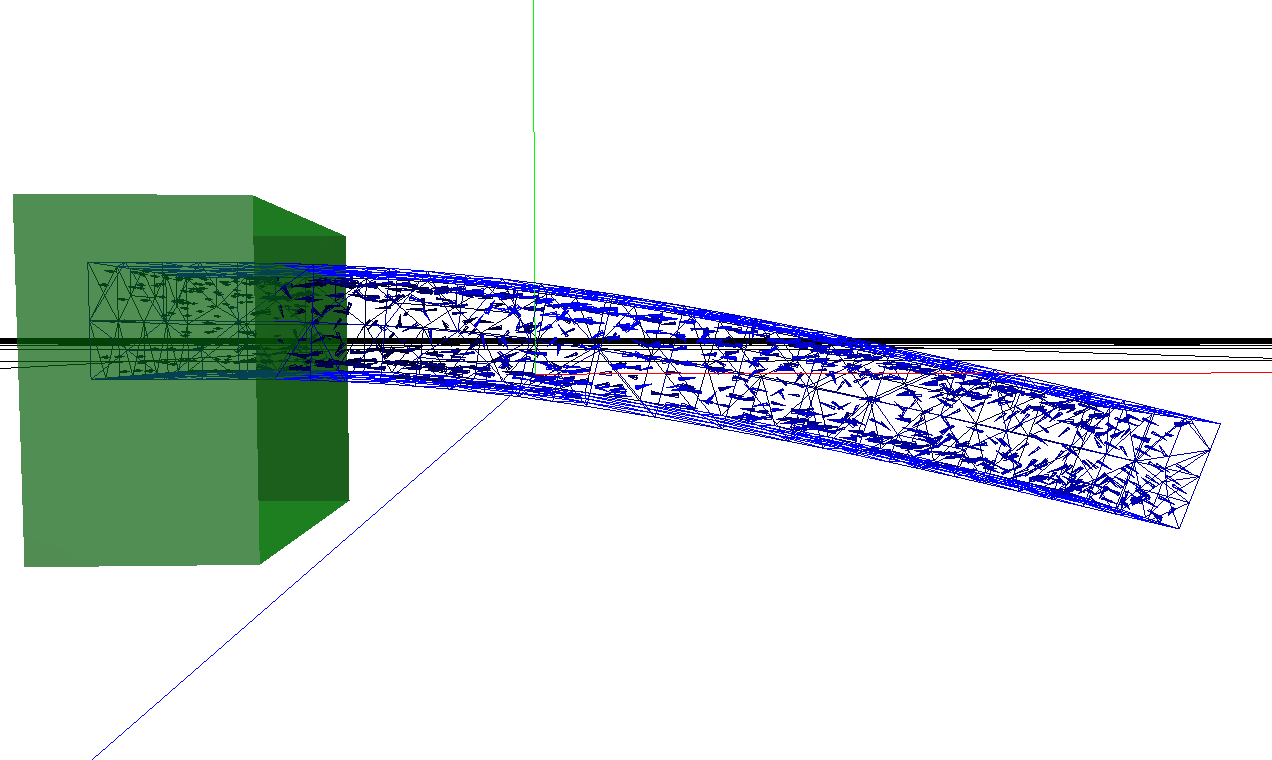
\includegraphics[width=12cm]{./images/helper_tools_tensor_visualization_0.png}
\caption{Beam with tensor visualization.}
\label{fig:tensor_visualization_with_planes}
\end{figure}

It can be difficult to interpret the tensor visualization especially
from a distance as illustrated in figure
\vref{fig:tensor_visualization_with_planes} where the scenario is a
beam fixed in one end with external forces pulling it down at the
other end.
But a closer look often reveals a pattern as illustrated on figure
\vref{fig:tensor_visualization_with_planes_closeup}. Notice that we
cannot determine the sign of the maximum principal stress direction,
this explains the opposite directions of the visual entities.
The principal
directions of the stress tend to point in a horizontal direction in
the top and bottom of the beam which corresponds to the tension and
compression in these directions. In the middle of the beam the stress
directions seem undetermined which in fact is the case when we
consider the magnitude of the stress alternating around zero in this
area.


\begin{figure}
  \centering
  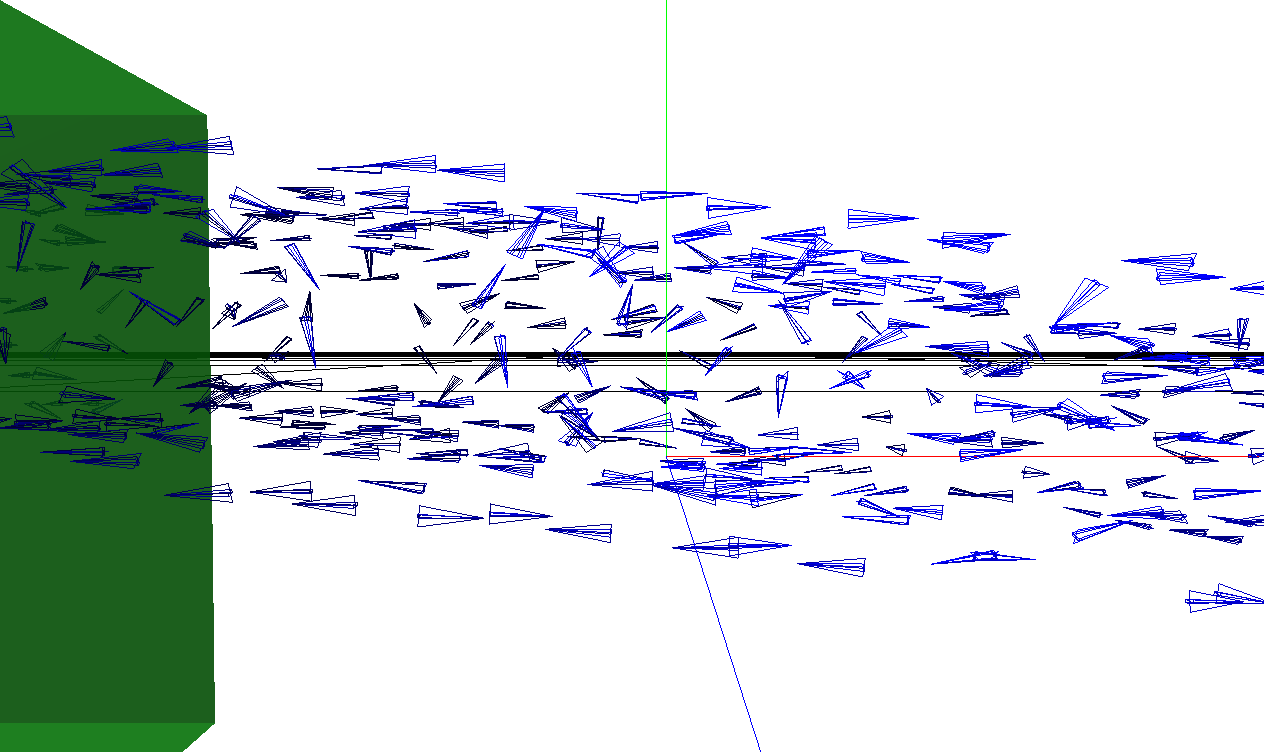
\includegraphics[width=12cm]{./images/helper_tools_tensor_visualization_1.png}
\caption{A closer look of the tensor visualization reveals a pattern.}
\label{fig:tensor_visualization_with_planes_closeup}
\end{figure}

